Z notranjo matriko in koeficienti popačenja lahko nepopačimo slike, zajete z isto kamero. Naslednja koda je iz \texttt{undistort.py}

\subsection{Nalaganje parametrov}
Tako kot smo jih shranili, lahko naložimo notranjo matriko in koeficiente popačenja s funkcijo numpy \texttt{np.load()}.

\begin{lstlisting}[language=Python, caption={Nalaganje parametrov},captionpos=b]
mtx = np.load('intrinsic.npy')
dist = np.load('distCoeff.npy')
\end{lstlisting}

\subsection{Nova optimalna matrika kamere}
Ta del ni obvezen. Z uvedbo parametrov prostega skaliranja alfa lahko nadziramo, koliko piksli izvorne slike se ohrani. Z drugimi besedami, z dajanjem različnih vrednosti za alfa nadzorujemo, koliko črnih piksli vidimo na robovih (1 vse, 0 nič). To matriko ustvarimo z \texttt{cv.getOptimalNewCameraMatrix(mtx, dist, (w, h), alpha)}

\begin{lstlisting}[language=Python, caption={Računanje nova optimalna matrika kamere},captionpos=b]
h,  w = img.shape[:2]
alpha = 0
newcameramtx,roi = cv.getOptimalNewCameraMatrix(mtx,dist,(w,h),alpha)
\end{lstlisting}

\subsection{Nepopačenje}
Za da izvedimo nepopačenja uporabimo \texttt{cv.undistort(img, mtx, dist, None, newcameramtx)}

\begin{lstlisting}[language=Python, caption={Nepopačenje slik},captionpos=b]
dst = cv.undistort(img, mtx, dist, None, newcameramtx)

cv.imshow('dst', dst)
cv.waitKey()
\end{lstlisting}

\begin{figure}[htp]

\centering
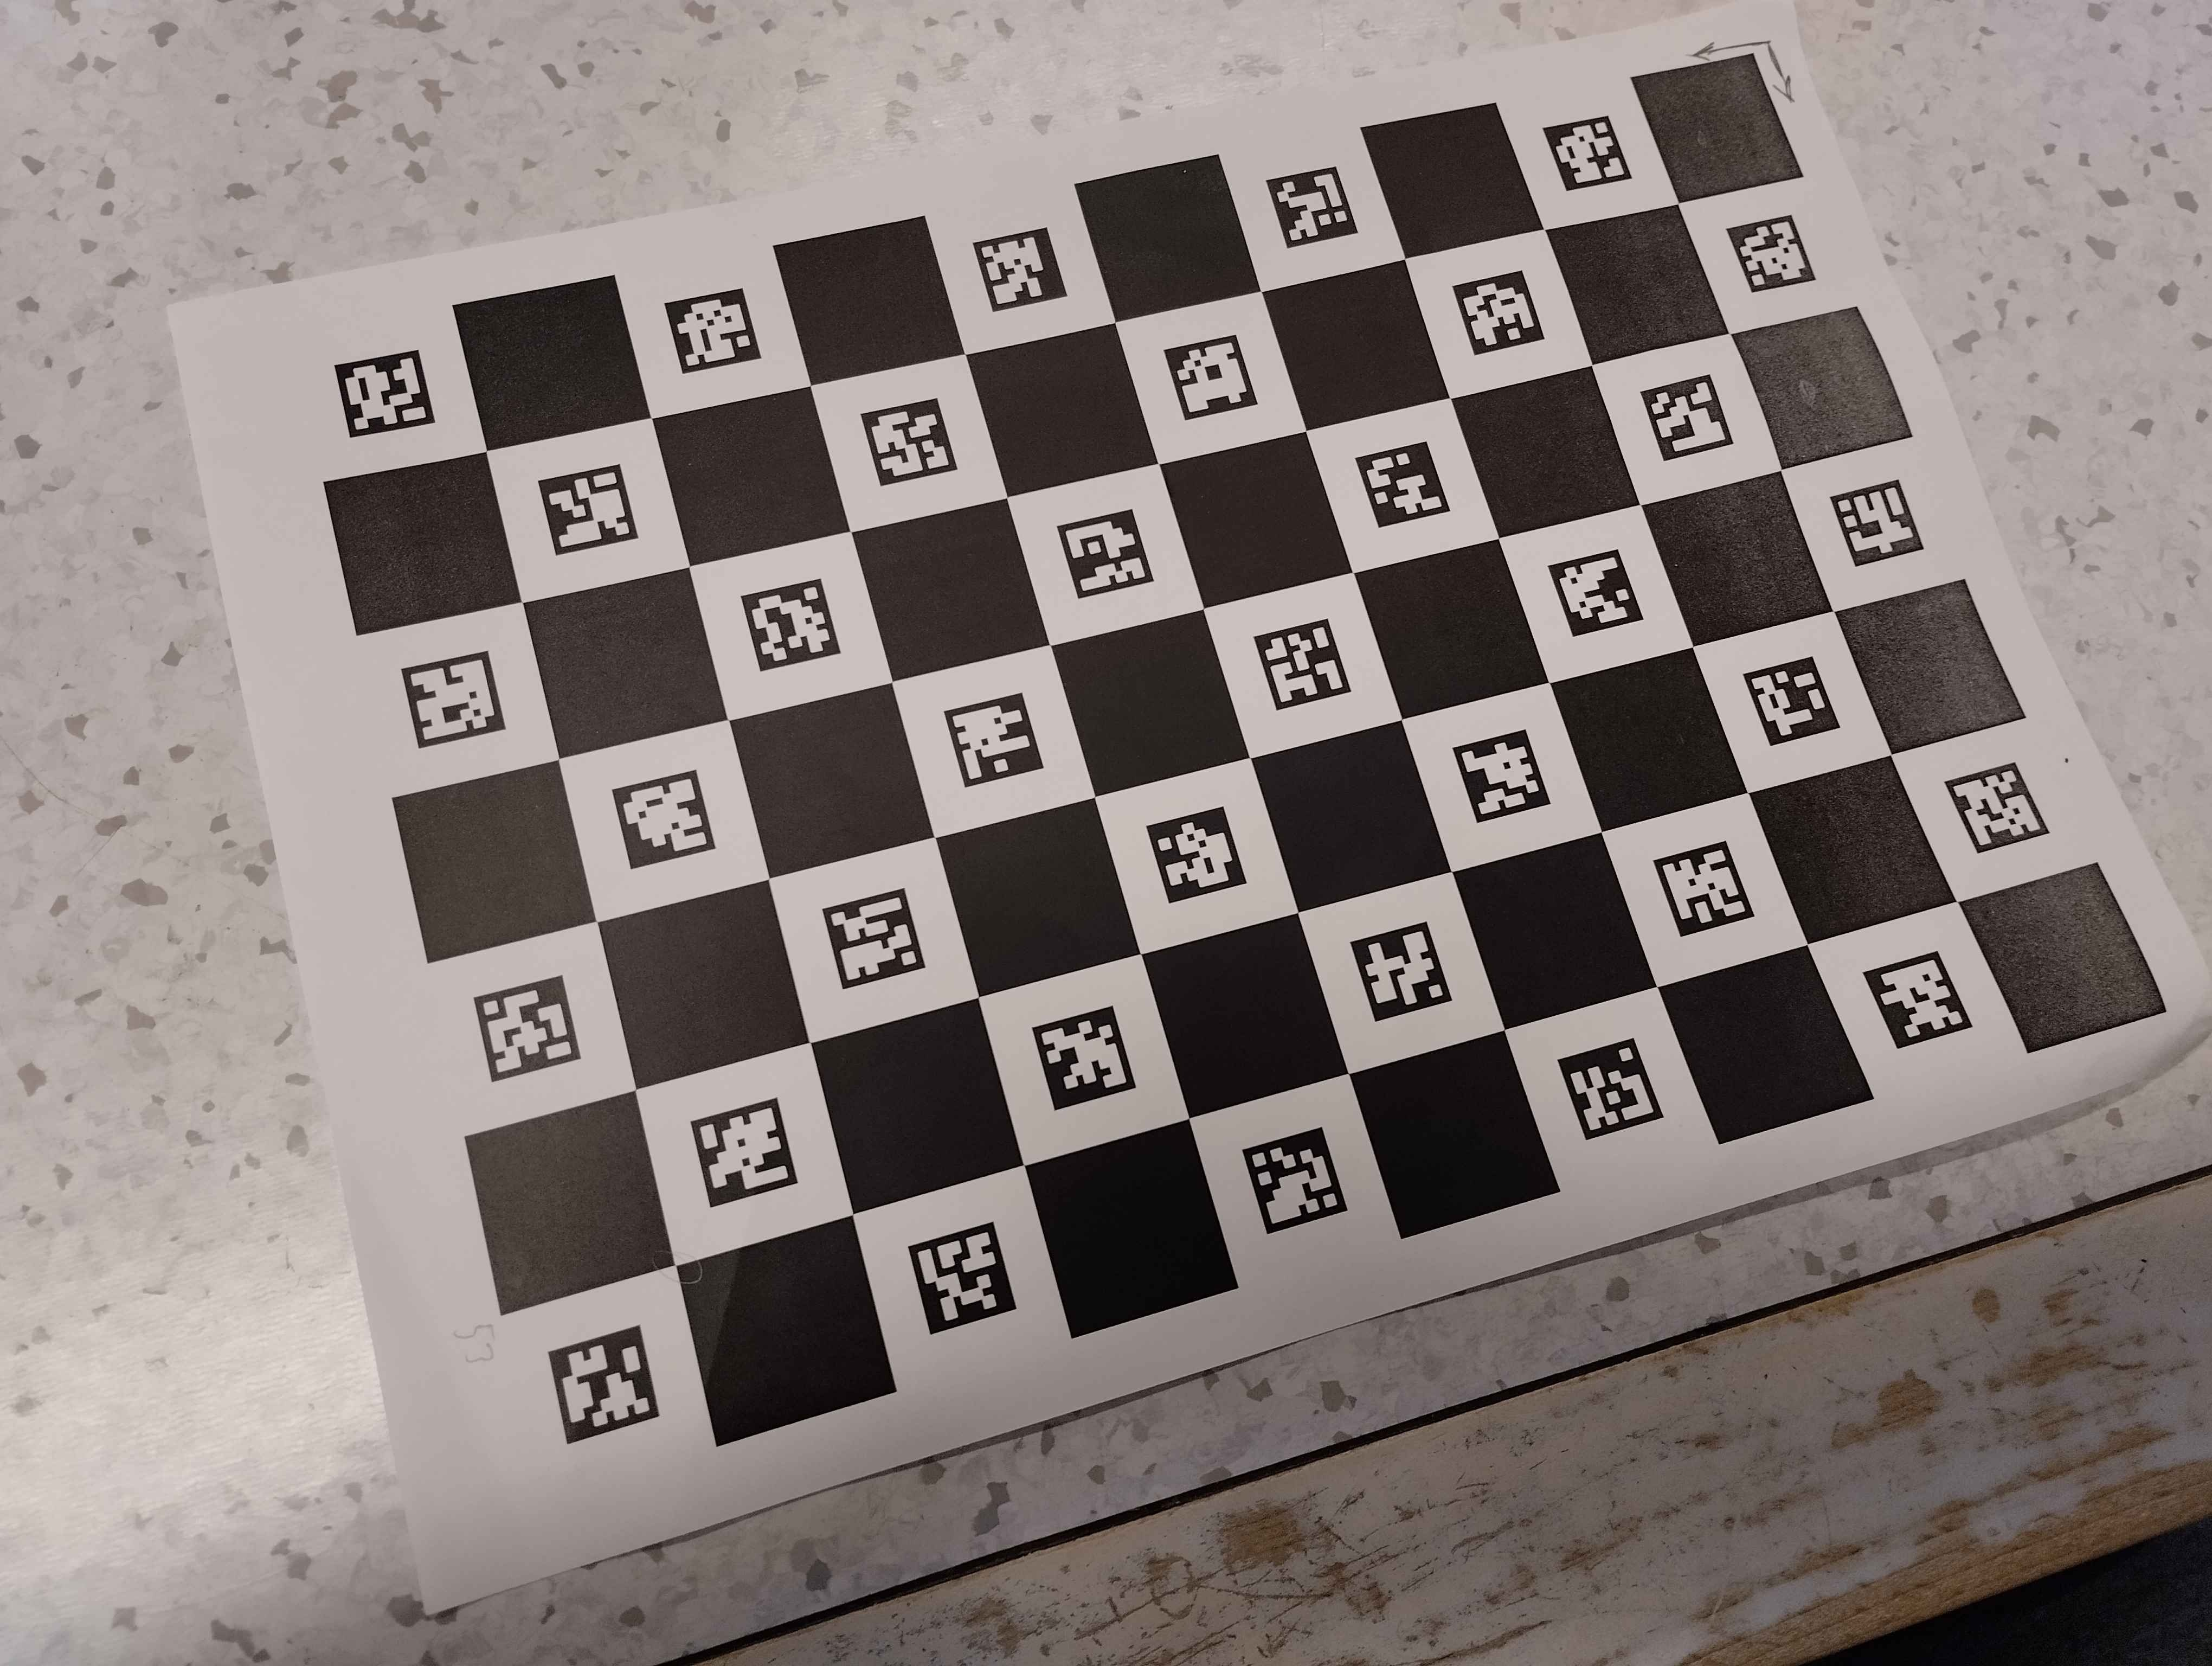
\includegraphics[width=.3\textwidth]{imgs/alphaorg.jpg}\hfill
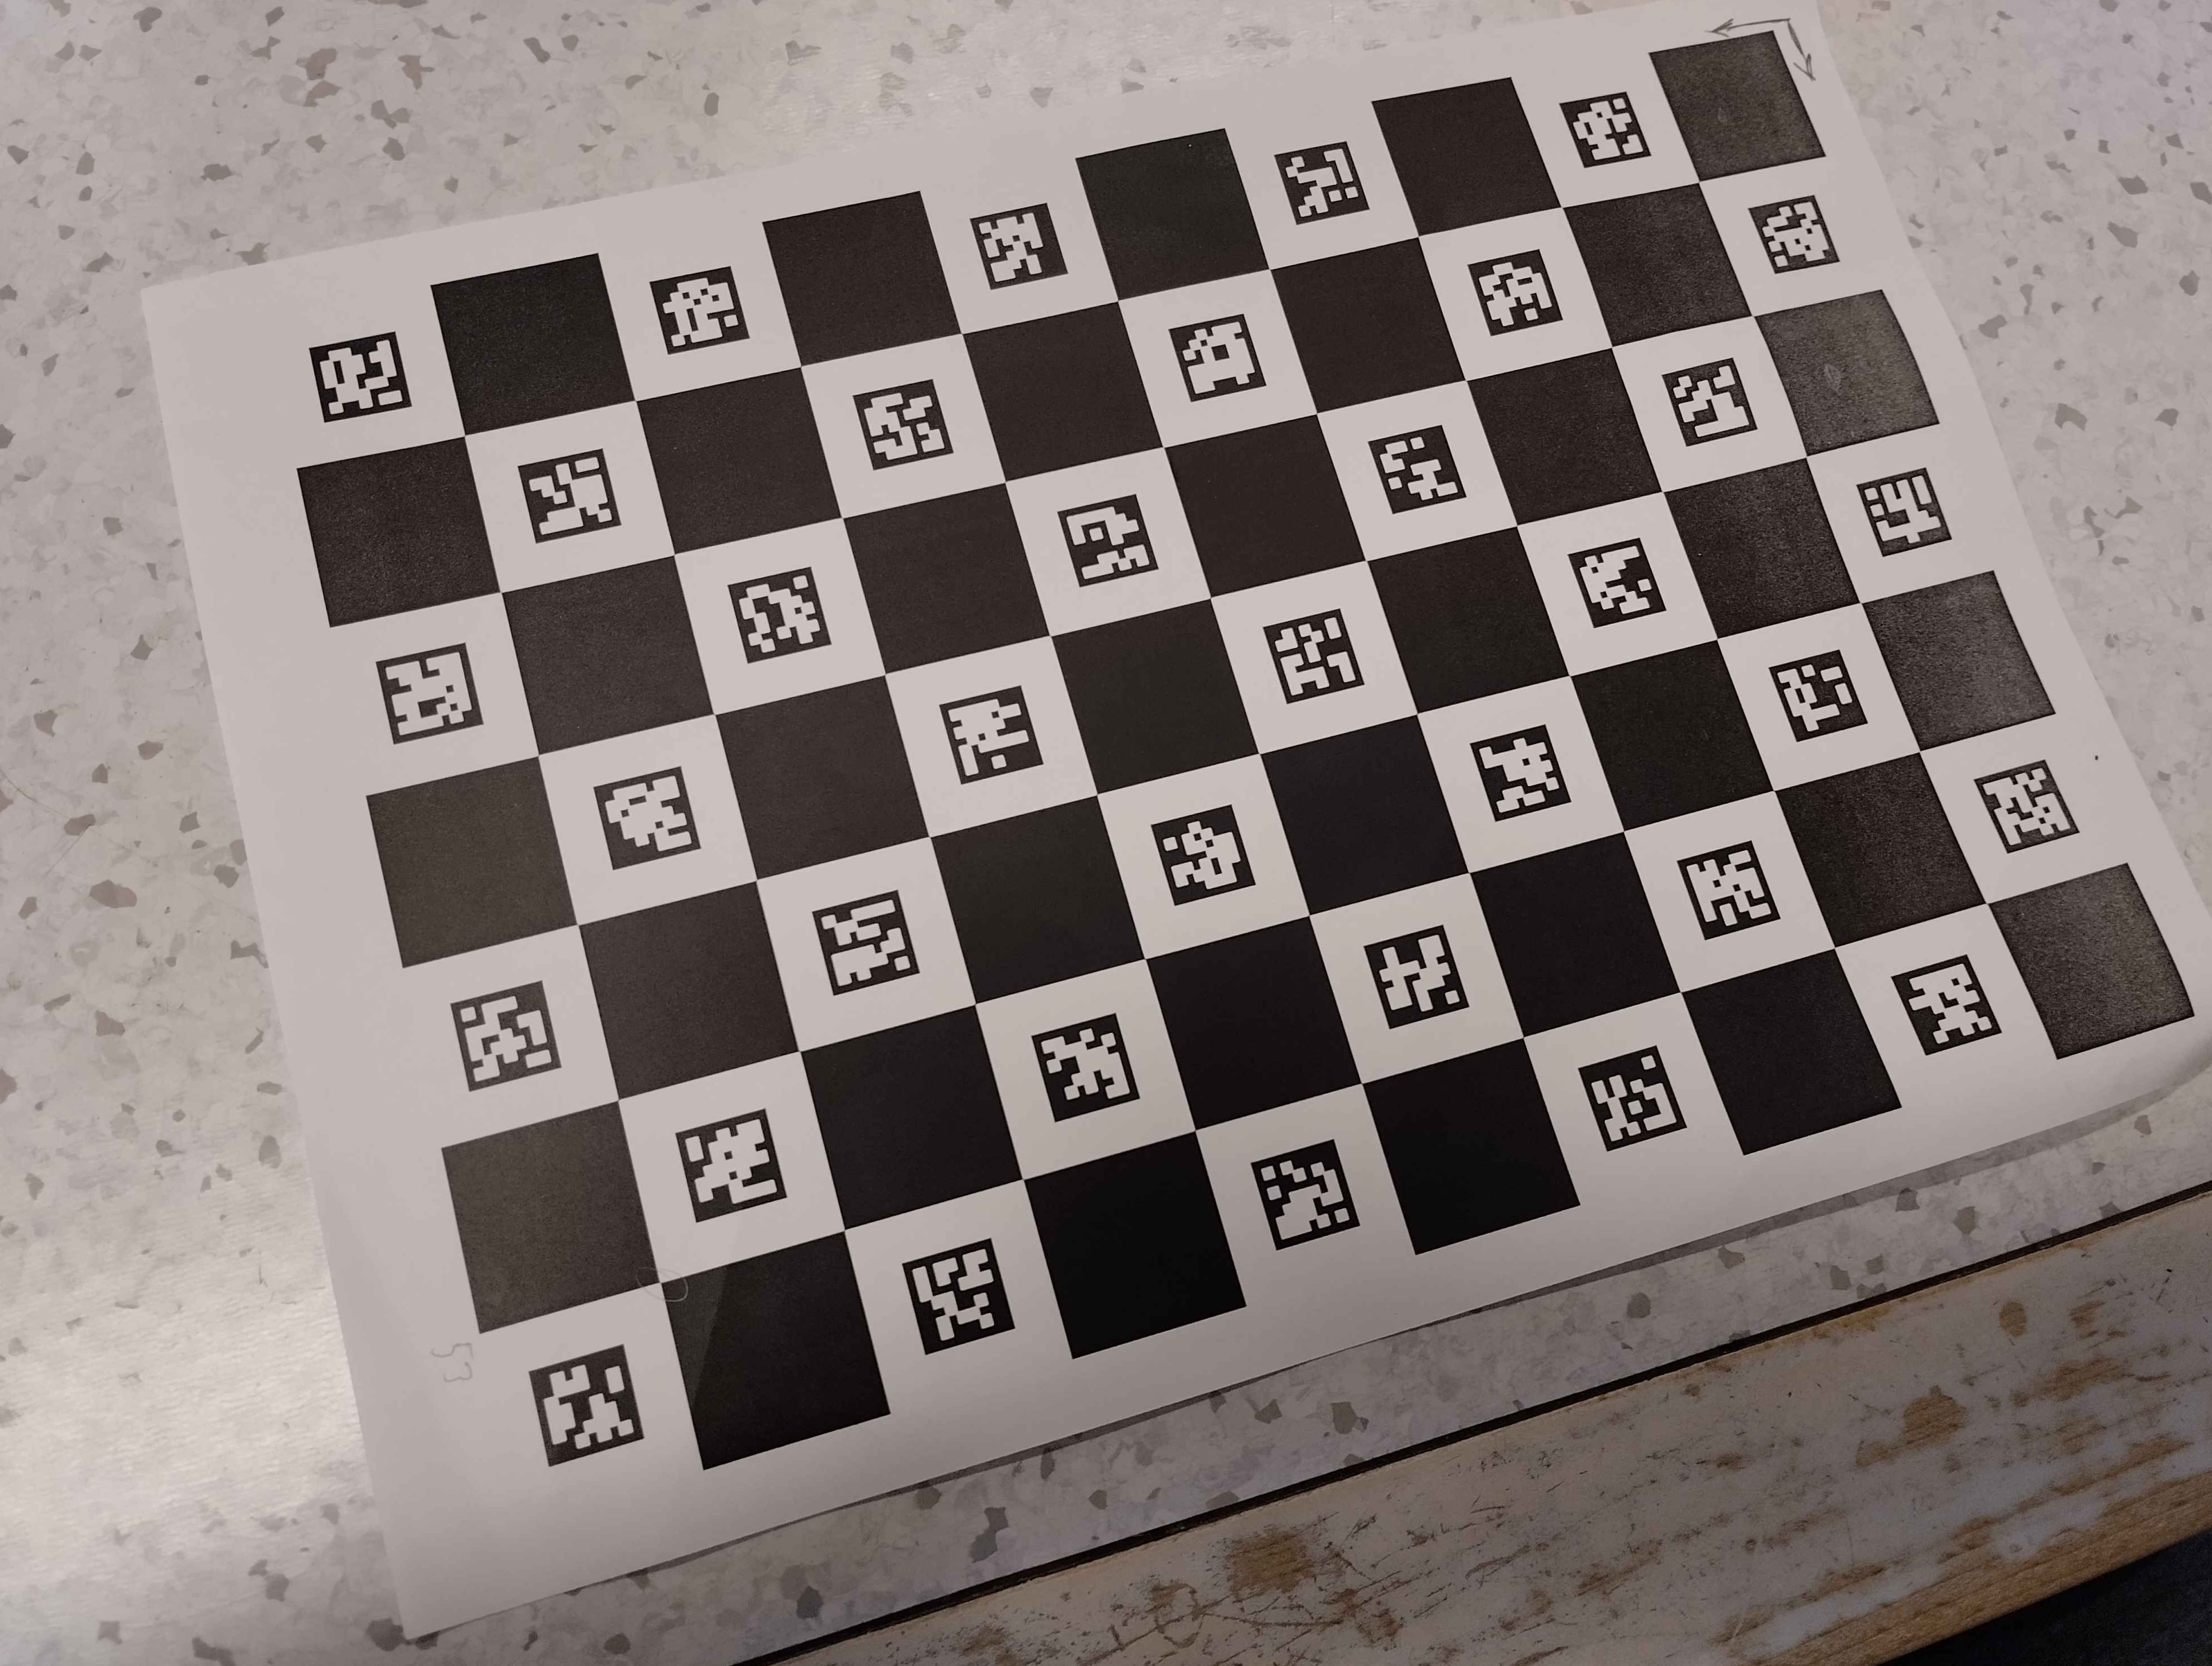
\includegraphics[width=.3\textwidth]{imgs/alpha0.jpg}\hfill
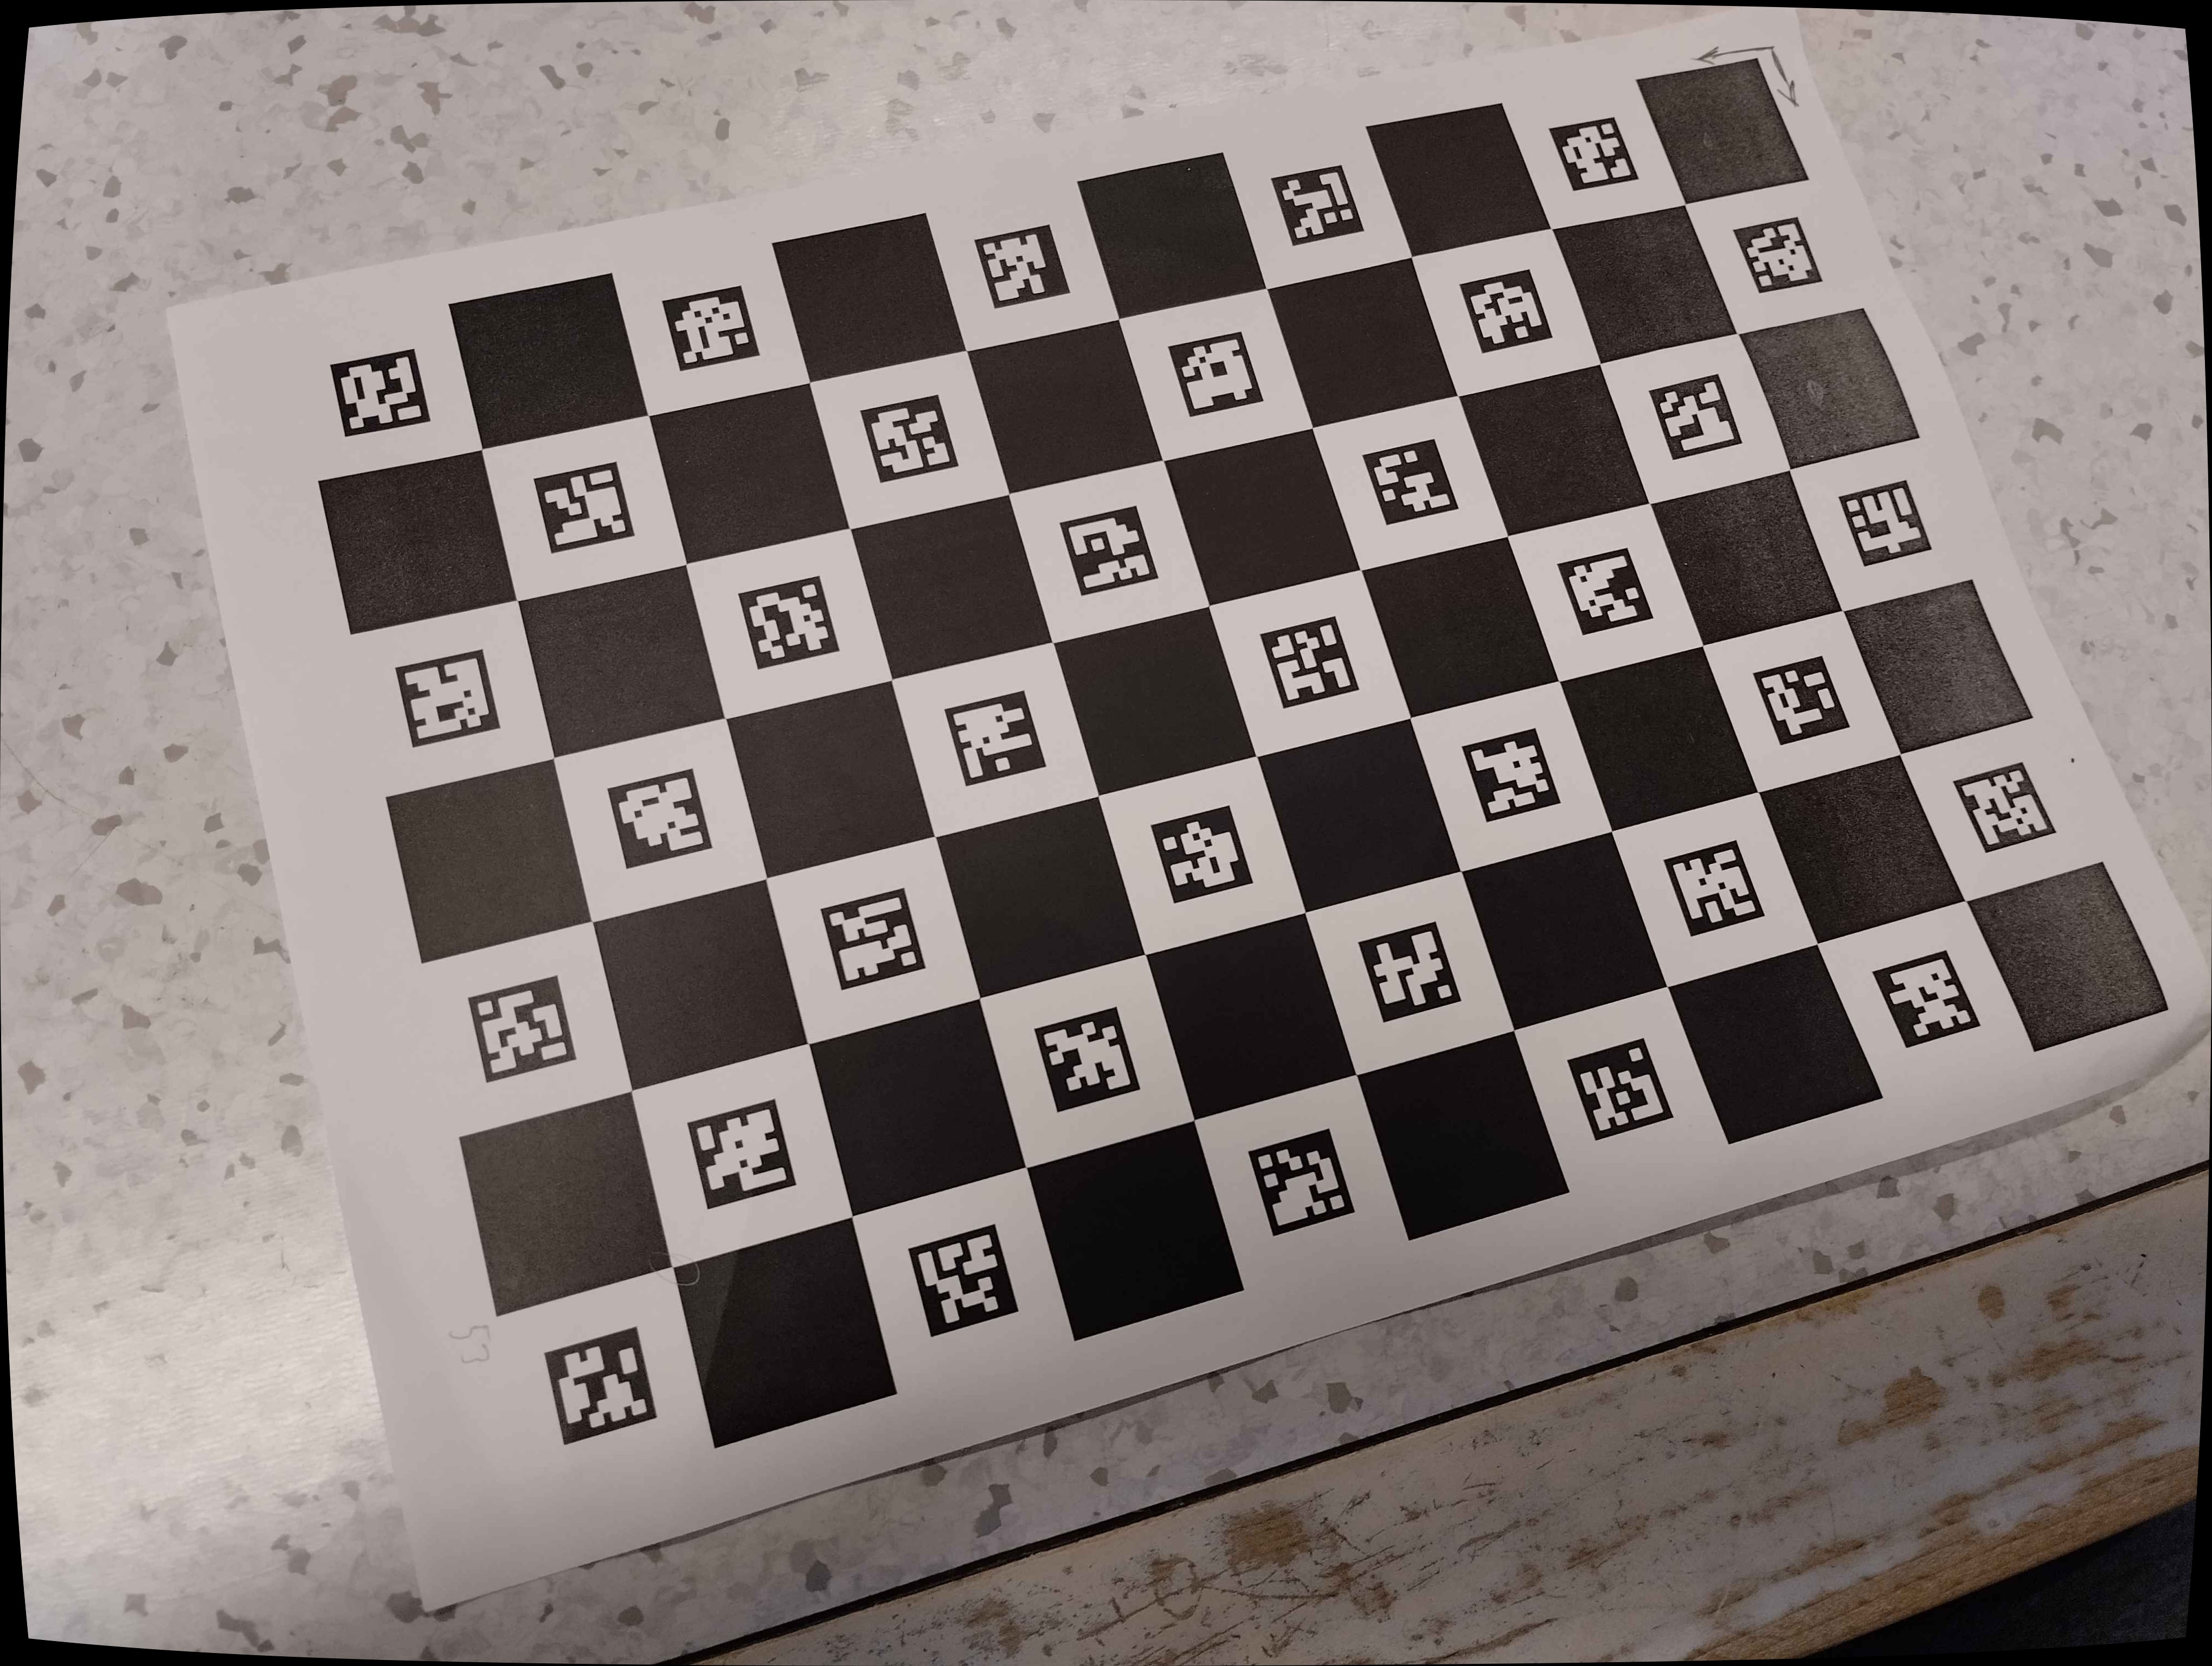
\includegraphics[width=.3\textwidth]{imgs/alpha1.jpg}

\caption{Rezultati: a) original, b) alpha=0, c) alpha=1}
\label{fig:figure3}

\end{figure}